\section{Date: 2026-08-26}
\noindent \textbf{Series ID: SFTPINDM114SFRBSF} 

\noindent This series is titled San Francisco Tech Pulse (DISCONTINUED) and has a frequency of Monthly. The units are Index Jan 2000=100 and the seasonal adjustment is Seasonally Adjusted.The observation start date is 1971-04-01 and the observation end date is 2020-03-01.The popularity of this series is 9. \\ 

\noindent \textbf{Series ID: CGMDLW2564} 

\noindent This series is titled Civilian Labor Force - College Graduates - Master's Degree, 25 to 64 years, Women and has a frequency of Monthly. The units are Thousands of Persons and the seasonal adjustment is Not Seasonally Adjusted.The observation start date is 2000-01-01 and the observation end date is 2026-07-01.The popularity of this series is 1. \\ 

\subsection{Raw Regression}
\noindent Regresses the two series against each other directly. A significant result here can come just as easily from both series sharing a long-run trend as from any real relationship.

\begin{center}
\begin{tabular}{lclc}
\toprule
\textbf{Dep. Variable:}                 & value\_fred\_CGMDLW2564 & \textbf{  R-squared:         } &     0.100   \\
\textbf{Model:}                         &           OLS           & \textbf{  Adj. R-squared:    } &     0.096   \\
\textbf{Method:}                        &      Least Squares      & \textbf{  F-statistic:       } &     26.65   \\
\textbf{Date:}                          &     Wed, 26 Aug 2026    & \textbf{  Prob (F-statistic):} &  5.10e-07   \\
\textbf{Time:}                          &         12:24:10        & \textbf{  Log-Likelihood:    } &   -2072.8   \\
\textbf{No. Observations:}              &             243         & \textbf{  AIC:               } &     4150.   \\
\textbf{Df Residuals:}                  &             241         & \textbf{  BIC:               } &     4157.   \\
\textbf{Df Model:}                      &               1         & \textbf{                     } &             \\
\textbf{Covariance Type:}               &        nonrobust        & \textbf{                     } &             \\
\bottomrule
\end{tabular}
\begin{tabular}{lcccccc}
                                        & \textbf{coef} & \textbf{std err} & \textbf{t} & \textbf{P$> |$t$|$} & \textbf{[0.025} & \textbf{0.975]}  \\
\midrule
\textbf{const}                          &    3082.1539  &      563.746     &     5.467  &         0.000        &     1971.655    &     4192.653     \\
\textbf{value\_fred\_SFTPINDM114SFRBSF} &      34.1431  &        6.614     &     5.162  &         0.000        &       21.115    &       47.172     \\
\bottomrule
\end{tabular}
\begin{tabular}{lclc}
\textbf{Omnibus:}       &  8.541 & \textbf{  Durbin-Watson:     } &    0.010  \\
\textbf{Prob(Omnibus):} &  0.014 & \textbf{  Jarque-Bera (JB):  } &    8.940  \\
\textbf{Skew:}          & -0.458 & \textbf{  Prob(JB):          } &   0.0114  \\
\textbf{Kurtosis:}      &  2.789 & \textbf{  Cond. No.          } &     609.  \\
\bottomrule
\end{tabular}
%\caption{OLS Regression Results}
\end{center}

Notes: \newline
 [1] Standard Errors assume that the covariance matrix of the errors is correctly specified.

\begin{figure}
\centering
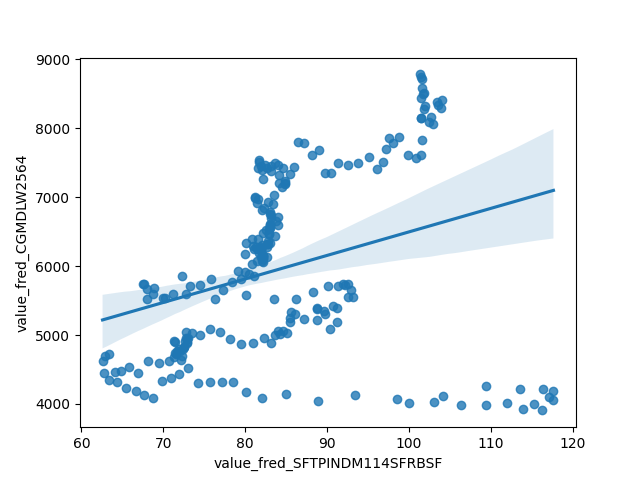
\includegraphics[scale = 0.9]{plots/plot_2026-08-26.png}
\caption{Raw Regression Plot for 2026-08-26}
\end{figure}
\newpage
\subsection{Detrended Regression}
\noindent Regresses the residuals of each series after removing its own linear time trend, so a shared trend can no longer drive the result on its own. A relationship that stays significant here is better evidence of a genuine link between the two series.

\begin{center}
\begin{tabular}{lclc}
\toprule
\textbf{Dep. Variable:}                            & value\_fred\_CGMDLW2564\_detrended & \textbf{  R-squared:         } &     0.136   \\
\textbf{Model:}                                    &                OLS                 & \textbf{  Adj. R-squared:    } &     0.132   \\
\textbf{Method:}                                   &           Least Squares            & \textbf{  F-statistic:       } &     37.94   \\
\textbf{Date:}                                     &          Wed, 26 Aug 2026          & \textbf{  Prob (F-statistic):} &  3.04e-09   \\
\textbf{Time:}                                     &              12:24:10              & \textbf{  Log-Likelihood:    } &   -1604.9   \\
\textbf{No. Observations:}                         &                  243               & \textbf{  AIC:               } &     3214.   \\
\textbf{Df Residuals:}                             &                  241               & \textbf{  BIC:               } &     3221.   \\
\textbf{Df Model:}                                 &                    1               & \textbf{                     } &             \\
\textbf{Covariance Type:}                          &             nonrobust              & \textbf{                     } &             \\
\bottomrule
\end{tabular}
\begin{tabular}{lcccccc}
                                                   & \textbf{coef} & \textbf{std err} & \textbf{t} & \textbf{P$> |$t$|$} & \textbf{[0.025} & \textbf{0.975]}  \\
\midrule
\textbf{const}                                     &   -3.482e-11  &       11.508     & -3.03e-12  &         1.000        &      -22.668    &       22.668     \\
\textbf{value\_fred\_SFTPINDM114SFRBSF\_detrended} &       6.1602  &        1.000     &     6.159  &         0.000        &        4.190    &        8.130     \\
\bottomrule
\end{tabular}
\begin{tabular}{lclc}
\textbf{Omnibus:}       &  7.909 & \textbf{  Durbin-Watson:     } &    0.417  \\
\textbf{Prob(Omnibus):} &  0.019 & \textbf{  Jarque-Bera (JB):  } &    9.938  \\
\textbf{Skew:}          &  0.259 & \textbf{  Prob(JB):          } &  0.00695  \\
\textbf{Kurtosis:}      &  3.845 & \textbf{  Cond. No.          } &     11.5  \\
\bottomrule
\end{tabular}
%\caption{OLS Regression Results}
\end{center}

Notes: \newline
 [1] Standard Errors assume that the covariance matrix of the errors is correctly specified.

\begin{figure}
\centering
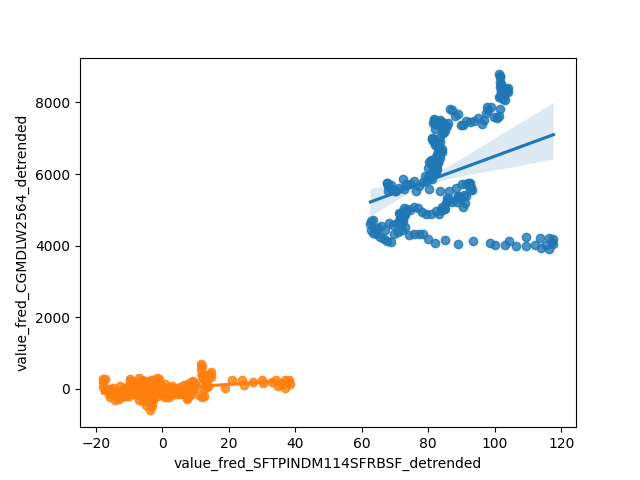
\includegraphics[scale = 0.9]{plots/plot_2026-08-26_detrended.png}
\caption{Detrended Regression Plot for 2026-08-26}
\end{figure}
\newpage
